%% \section{Overview}

%% [TODO put this to a separate file and come with a plan]

%% [Shall we put the assumptions/setup here?]

%% [Shall we put the interface here?]

%% [Give a table, summarize the interface]

%% % \subsection{Interface and Assumptions}
%%                                 % Giza is an erasure coding scheme for key/value stores and provide two operations: Put(Key, Value) and Get(Key), where Key and Value are arbitrary strings. Get(Key) returns the value of the latest Put for that key. (Add assumptions here + what giza is good for: Giza provides fault tolerance for non byzantine failures in an asynchronous network)


%% % operations  semantics
%% % put         
%% % get 
%% % get_stale

%% \subsection{State Machine Replication and Paxos}

%% \subsection{Erasure coding}

\section{Design}

This section will present the basic design of {\name}, including the overall architecture,
the metadata schemes, and the protocols for supported operations in {\name}. 

\subsection{Overview and challenges}

\begin{figure}[tp]
\centering
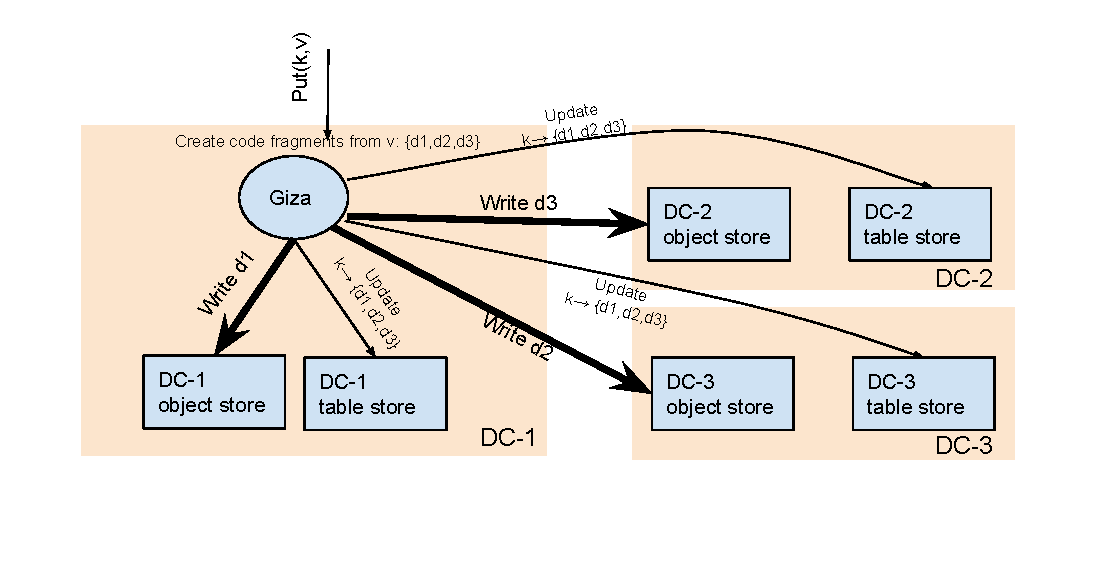
\includegraphics[width=0.5\textwidth]{fig/Giza}
\caption{Giza architecture\label{fig:arch}}
\end{figure}

\paragraph{Architecture}
{\name} is a global-scale cloud storage systems that span across many
datacenters in the world.  \name stores mutable, versioned objects.
~\Cref{fig:arch} shows the architecture of \name.  To support mutable coded
objects, \name separates the data path from meta-data path.  On the data-path,
object data is coded into several fragments, named by their content hashes, and
stored in the different DCs.   On the meta-data path, \name stores the set of
content hashes of coded fragments as the new version information for the object.

We take the approach to layer \name on top of existing cloud storage infrastructure. This 
provides two advantages.  First, doing so allows the rapid prototyping of \name by re-using 
mature, deployed systems.  Second, it simplifies the failure recovery and 
the deployment of \name, as \name servers are completely stateless and can be
readily integrated with the rest of the stateless cloud storage frontend.
Existing cloud storage systems have redundancy within a single data center, but
are not geo-replicated.  Thus, \name must explicitly provide cross data center
redundancy through coding and replication.  To write to an object, {\name}
stores coded fragments in cloud blob stores in different data centers, such as
Azure's blob store, or Amazon's S3.  Additionally, \name updates the object's
meta-data information (e.g.  versions, names of coded fragments for the new
content) in existing cloud tables and replicates them across several data
centers.  The number of coded fragments, and thus the set of data centers
storing object data, is configurable depending on the user desired tradeoff on
durability vs. cost.  The number of data centers to replicate the meta-data is
fixed at 3.

%blob service as building blocks, to store metadata and data respectively. This evolutional
%design allows {\name} to minimize footprint of new code. In fact, {\name} merely needs to replace the previous front-end
%module. With {\name} deployed, the user request comes in to the new frontend, where the new
%{\name} service will translate the user requests into a few metadata operations and data operations.
%
%In {\name}, both metadata and data are synchronously duplicated across different
%datacenters in order to tolerate datacenter failures. What is different between metadata
%and data is, metadata is fully replicated across a (usually smaller) set of datacenters using
%a tailored Fast-Paxos algorithm, persistent in the table service in each datacenter, thus
%tolerating a minority of failures; On the other hand, data in user request is encoded to
%a configurable number of fragments and shipped to a (usually larger) set of datacenters,
%persistent in the blob storage service. We refer the former as metadata path and the latter
%as data path.


\paragraph{Technical challenges}
In designing \name, we address three main technical challenges facing the basic approach.
\begin{enumerate}

\item {\it Building a strongly consistent, geo-replicated meta-data storage out of existing 
single-DC cloud tables.}  There are existing geo-replicated,
strongly-consistently storage systems (Cassandra, CockcoarchDB) that have been
built from the scratch.  However, we choose not to use them because we want to
keep \name servers stateless and keep all data and meta-data in existing
storage infrastructure that are operated by cloud providers. The common
technique to ensure strong consistency is to implement the Paxos protocol.  How
to implement Paxos using existing cloud storage APIs and achieve 
good performance in the cross-DC setting?

\item {\it Jointly optimizing the data and meta-data paths to achieve a single
cross-DC roundtrip for read/write operations.}  Under the naive approach, the
data and meta path are treated completely separately; a
\name node completes the data path first before starting on the meta-data path.
While doing so guarantees that data is durably written at multiple DCs before it becomes
readable, each read/write operation takes at least two cross-DC. Can \name 
combine data and metadata path operations to achieve a single cross-DC roundtrip?

\item {\it Performing garbage collection efficiently and promptly.}  When data is 
over-written and deleted, \name must remove obsolete data and/or meta-data from
the underlying cloud storage.  This is non-trivial because \name's garbage 
collection mechanism must be able to handle DC failures while ensuring data 
consistency and durability.

\end{enumerate}

%The separation of metadata path and datapath bring in the challenge that the consistency level
%could be violated with brutal yet flawed merge of the two. Our protocols described in later
%sections will guarantee the metadata path and data path together (especially when they are
%fully concurrent) will still provide a strong consistency insurance.
%


% A typical giza architecture for a data center includes the giza nodes, the Azure Blob Storage, and the Azure Table Storage. The giza nodes are the processing units of the Giza architecture and manages the data and the metadata. Furthermore the giza nodes participate in paxos rounds as coordinators. Figure 1 illustrates the architecture of Giza. Giza separates data from metadata and handles them on different paths. The data path is responsible for encoding the data and sending the data fragments across data centers. Each data fragment is stored in the corresponding DC’s Azure Blob Storage. The metadata path is responsible for storing the latest version of the data and the location of its data fragments. Giza uses a variant of the Paxos state machine replication (SMR) to maintain consistency of the metadata where each metadata server maintains a local copy of the replicated log. The replicated log is stored in the Azure Table Storage.

\subsection{Implementing Paxos using Cloud Storage APIs}

On the meta-data path, \name implements the Paxos protocol on top of existing cloud table storage, such 
as Amazon DynamoDB or Azure Tables.

\begin{figure}[tp]
\centering
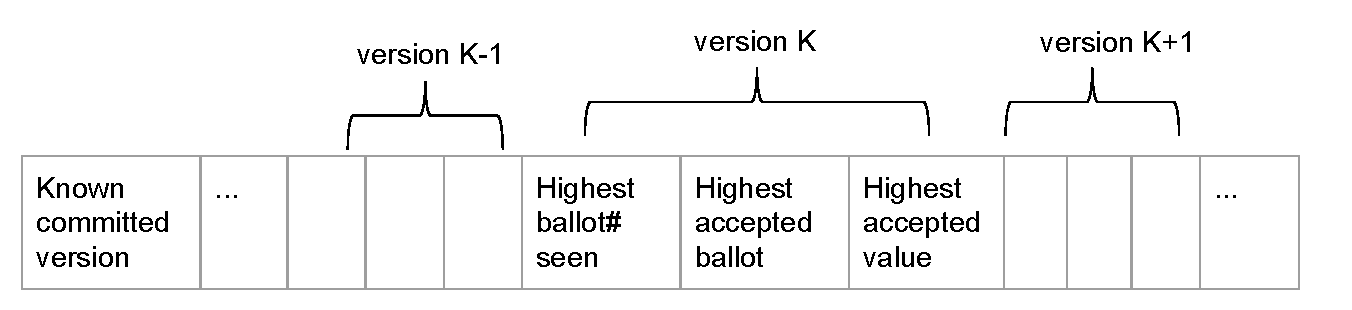
\includegraphics[width=0.5\textwidth]{fig/Giza_Metadata}
\caption{For each object, \name stores the Paxos protocol state and the object meta-data 
in a single row in the underlying cloud table.\label{fig:metadata}}
\end{figure}

{\bf Meta-data storage layout.}
\name uses the Paxos protocol to serialize the operation on each data object.  Thus, it 
must keep Paxos protocol state together with the metadata for each object. Instead of storing the Paxos state elsewhere, {\name} makes the design
choice to store the Paxos state together with the metadata itself,
one row per object, with a dynamic number of columns. The layout of each row is
shown in~\Cref{fig:metadata}.  

Each \name write operation generates a new
object version, which is associated with an instance of Paxos invocation to
ensure consistency in the event of races among multiple writers and failures.
Thus, the meta-data contains a triplet of columns for each version of object
(~\Cref{fig:metadata}). The triplet includes {\tt highest\_proposal\_seen},
{\tt highest\_accepted\_proposal}, and {\tt highest\_accepted\_value}.  These
fields are necessary for running each instance of Paxos.  The {\tt
highest\_accepted\_value} for a version contains the meta-data information for
coded data fragments; these include the name of each fragment, wehther it is
one of the original or parity fragments, and which DC it is stored at. 

{\name} uses the {\tt known\_committed\_version} to represents the highest 
version number known to have committed by Paxos.  This provides a hint on the latest 
modification rather than a decisive answer, since there might be a higher
\emph{ongoing} version that has just reached agreement.  

{\bf Meta-data Write.}
The metadata path begins with
choosing a proper version number to run the Fast-Paxos~\cite{fastpaxos} algorithm. The version number needs
to be the next version to the most recently committed version.  While it is safe to use an outdated
version (in which case the {\name} node will notice its mistake later and retry with a higher one),
but it is unsafe to choose a higher one. {\name} node finds the proper version in an
optimistic fashion. Specifically, it reads the {\tt known\_committed\_version} from the
table in its local DC, then uses the next higher number as the chosen version number to 
invoke the corrresponding Fast Paxos instance.

With the version number chosen, the {\name} node sends out a PreAccept request to the cloud table
in each DC. The request is an atomic conditional update, if there are no other 
requests on that version, the write for the PreAccept request will be successful, otherwise
the corresponding write will be rejected by the table service. If the {\name} node receives a fast quorum of successful PreAccept requests, the
corresponding version is considered to have been committed. The {\name} node asynchronously 
sends out Commit requests to all DCs to modify the {\tt known\_committed\_version} field to 
reflect the recently committed version.  The commit request is also a
conditional write; the write only succeeds if the current {\tt
known\_committed\_version} is not does not contain a higher version.

The above described metadata update involves only one cross-DC roundtrip (the
commit is done in the background, so only the PreAccept is counted as part of
the critical path) and is referred to as the fast path.  When there is no
contention, the fast path always succeeds. 

In the case of contention, the fast-path may not succeed, i.e. the {\name} node
cannot collect a fast quorum of successful PreAccept requests. The contention
may come from concurrent updates to the same object, or a {\name} node trying
to recover from failures by re-committing the same or a different value to an
ongoing version.  In this case, {\name} enters what is referred to as
\emph{slow path} to perform classic Paxos in order to guarantee safety in case of
contention.

On the slow path, the {\name} node first picks a distinguished ballot number
and then sends out a Prepare request to write that ballot to all metadata
tables and wait for at least a majority of responses. The Prepare request is a conditional
write operation; the write operation succeeds if the {\tt highest\_ballot\_seen} is not higher than 
the ballot in the Prepare request and it also returns the entire row as a result.
Upon a majority of successful replies, the {\name} needs to pick a value to try to commit.
The rules for picking the value is as follows. First it looks for the highest accepted ballot
in the replies. If there is one, the value from the reply is picked. If there is no accepted
value, but there is pre-accepted value, the {\name} node will pick the pre-accepted value
that appears more than others (if any) from the replies. If there is neither pre-accepted
nor accepted value. The {\name} node can pick any value it wants, e.g. the value it receives
from client or a \texttt{no-op} placeholder in failure recovery.

After the {\name} node picks a value, it sends out Accept request to all metadata tables.
The accept request is a conditional update; it succeeds in writing the {\tt
highest\_accepted\_ballot} and {\tt highest\_accepted\_value} if neither {\tt
highest\_ballot\_seen} and {\tt hightest\_accepted\_ballot} are larger.  If a
majority of Accept requests succeeds, the \name node considers the
corresponding meta-data write as complete and may return to the client.
Additionally, a commit phase similar to one described above is launched in
background.

{\bf Metadata Read.}
To read the \emph{latest} metadata of an object, it is not sufficient that the \name node 
only reads the corresponding metadata row from its local DC, since the local DC
might not be part of the majority quarum that has accepted the latest value.
The \name node reads from the metadata rows from all three DCs.  If a majority
rows have matching {\tt known\_committed\_version} $k$ and have not accepted
any value for a version higher than $k$, then the \name node returns the
metadata for version $k$ to the client.

If unfortunately the {\name} node observes a higher version with accepted value in the
replies, it needs to try a slowpath in the put operation above to confirm on that version
because it could possibly be considered committed once before. After it succeed in
the slow path, the {\name} node needs to re-launch the datapath to retrive the data
fragments of the newer version and abandon the old ones. This serialized metadata and
datapath case typically happens when there is concurrent read and write on the same
object, which is rare in our workload.

\sm{ Hi Daniel, just want to confirm, is this what you do now? Only one accepted
  in higher version will invalidate the optimistic read}


%The metadata row is replicated in a number of datacenters using a variant of Fast-Paxos
%algorithm. Instead of storing the states of Fast-Paxos elsewhere, {\name} made a design
%choice to use the metadata row itself as a durable space to hold the Fast-Paxos states.
%The advantage of this choice is that {\name} can reuse the table service as the persistence
%layer for the state machine replication, making {\name} nodes themselves stateless. As a
%result, {\name} node has much less to worry about failure recovery. When a {\name} node
%is (suspiciously) failing, a new {\name} node can be launched as an replacement without
%doing extra work to nullify the previous node. The new node can directly access the table
%service to work. 

%The metadata for each object includes the latest modification to that object using a versioning scheme. The highest version corresponds to the latest modification and the decided value for the version. In addition, the metadata also includes the location of the data fragments for the latest version. The metadata is replicated using a variant of the Paxos state machine replication. Instead of having a single log recording all the executions, each object has a corresponding paxos log. Giza uses the fault-tolerant Azure Table to store the metadata where each entry in the table corresponds to an object. Figure 2 illustrates the schema of the metadata table. 

\subsection{Joint optimization of Data and Meta-date Operations}

The data path of \name is straighforward: the \name node encodes the data to $k$ original
fragments and $m$ parity fragments. $k$ and $m$ are configurable. Then the node
computes a content hash for each fragment, and use the hash value as key to
write each fragment to a separate datacenter.  In the naive combination of data
path and metadata path, the \name node serializes the two paths,
resulting in at least two cross-DC roundtrips.  We design \name to reduce
latency by running the data and metadata paths in parallel.  This is
potentially problematic because either the data or metadata path could fail
while the other one succeeds.  Below, we describe the end-to-end client
operations and how they address this challenge.

{\name} supports three operations: put, get and delete. All of them require a key as
an argument to identify an object. put takes object content as an extra argument, get
returns object content (null if non-exist) as result. A delete operation is processed
as a special write, putting a tombstone in the object's metadata. The actual recycling
of disk space happens at garbage collection, which will be described in ~\Cref{sec:xxxx}.

{\bf The Put Operation:}
After calculating the coded framents, the \name node launches both data and
metapath paths in parallel.  To ensure that data is written durably in multiple
DCs, the \name node waits for both the metadata and the data path to finish
before returning to the client.  Furthermore, the \name node only starts 
the Paxos commit phase after the data path completes. In other words, \name 
ensures that {\tt known\_committed\_version} only refers to fragments
that have been successfully written to their intended DCs.
 
{\bf The Get Operation:}
The naive way to perform Get is to first reads the latest metadata and then retrieves 
the coded framents. 
To cut down cross-DC latencies, {\name} chooses an optimistic approach to parallelize the metadata and data path.
On a Get request, the {\name} node first reads from the corresponding metadata row from the table in the local DC
to obtain the {\tt known\_committed\_version} and the corresponding coded 
fragments location information. Then it immediately starts reading the data fragments from different
datacenters.  Separately, the {\name} launches a regular metadata read to validate that the version it uses is actually
the correct latest version. If the validation fails, i.e. the \name node
has to redo its data path by fetching a different set of data fragments,
resulting in wasted efforts in its previous data fetch.  Such potential waste
only happens when there is concurrent read and write on the same object, which
is rare in our workload.

Because the data and metadata paths are performed in parallel during Puts,
there is a rare case that the data fragments for the latest committed version
have not been written to the blob storage at the time of read. This happens if 
the metadata path in the corresponding Put finishes before the data path. In
this case, the {\name} node in the get operation needs to fall back to read the
previous version, up to the version specified in {\tt
known\_committed\_version} $k$ as $k$ is only written when the corresponding
data path has completed.

\sm {
  Hi Daniel, can you give me a few details about the hashing? e.g. hashing method,
  hashing result size, collision rate, etc.)
}

\subsection{Garbage Collection}
Because {\name} keeps writing new version metadata to table service and data fragments
to blob storage service, it needs to garbage collect on outdated versions to recycle
storage space. Moreover, the garbage collection also needs to free the space marked as
tombstone by the delete operation.

Recycling the old versions data includes deleting the data and parity fragments and
truncating the columns for the old versions in the metadata row. Garbage collection
for an object follows three steps: 1) read the metadata row and get the columns to
delete based on the \texttt{hightest\_committed\_version}. 2) send delete requests to
blob storage service to delete the data. 3) remove the columns for the old versions
in the table service. The second step has to happen before the third in case that the
garbage collection process is interrupted and the data fragments may become ``orphans''
without proper metadata to point to them in the table service.

After a delete operation, {\name} sees the row marked as tombstone by a special column.
Now it needs to remove the entire row, which requires extra care. Otherwise if removed
brutally, another put operation on the same key may bring the system into an abnormal
state. The new put operation will start with the initial version again, which could
violate some of the metadata (with a higher version before the deletion) if the removing is still in
process. Therefore, {\name} chooses to use two-phase commit when to remove the metadata
row. In the first phase, it marks the rows in all datacenters as ``prepared\_to\_delete''.
After this any other get or put operations are temporarily disabled on this row. Then
in the second phase, all the rows are actually removed from the table service. The
disadvantage for this approach is that it requires all datacenters online. Any crashed
datacenter or network partition may pause the process and makes the row unavailable
(but can still continue or recovered after the failure is eliminated). 



% \subsection{Giza Workflow}
% Because of the high WAN RTT, Giza’s primary goal is to minimize the number of round trips in its put and get critical paths while maintaining strong consistency semantics. By approaching this problem with multiple iterations, we were able to reduce the original 3  WAN RTT to 1 WAN RTT in most cases, dramatically reducing the put and get latency.

% \subsubsection{3 RTT Put and Get}
% Figure 3 illustrates the workflow of a typical Put operation. When a client issues a Put command, Giza first queries its local metadata to identify a most likely latest version of the object. It then starts a paxos round for the version. A paxos round is broken down into two phases: the prepare phase and the accept phase. Giza runs the data path first, where the object is erasure encoded and the data fragments are sent to the corresponding data centers. (Here, we have to write this information down in case of giza node failure right). When the data path returns successfully, Giza proceeds to run the metadata phase which incurs two round trips.
% \par 
% During the Get path, Giza runs the metadata phase first to get the location of the data fragments. To ensure a consistent latest version of the data, Giza runs a paxos round for get on the object’s entry log. When this succeeds, Giza runs the datapath and receives enough data fragments to reconstruct the original data before returning to the client. Both the Put and Get incurs two rounds in the metadata path and 1 round in the data path.

% \subsubsection{2 RTT Put and Get}
% We quickly realized that the separation of metadata path and data path allows for some parallelism. In particular, during the Put path, Giza can run the prepare phase of the metadata path in parallel with the data path. When prepare phase and the data path succeed, Giza runs the second phase of the paxos round. Once this round completes, Giza can return acknowledgement to the client. This brings the round trips down to 2 round trips in the optimal case.
% \par
% Furthermore, during Get, Giza can run the additional paxos round for the get operation in parallel with the data path get. This can be done by first optimistically assuming that the current highest entry of the object in its local entry log is in fact the highest version. Once this information is obtained, Giza can then proceed to get the data fragments while simultaneously validating the consistency of the latest version on the metadata path. If the assumption is correct, the Get incurs 2 round trips.

% \subsubsection{1 RTT Put and Get}
% We used the classical Paxos protocol for achieving consistency on our metadata path. [Introduce Fast Paxos and why this works in this case, should do this after reading in depth about Fast Paxos]. This reduces Giza’s put path to 1 round trip.
% \par
% In the Get Path, we realized that we can forego running the paxos round in some scenarios by including a learning phase on the non-critical path of Put. After acknowledging to the client’s put request, the coordinator giza node will send the accepted version and the version number as a committed entry for the object to the other participating giza nodes. This entry is used to serve as the highest committed version and will only override existing entry if the version is higher. During a client’s Get request, Giza first obtains the object’s row entry from the majority of the participating giza nodes. If the latest entry in the paxos log are consistent or not higher than the highest committed entry, then Giza can safely return the results obtained from the data path. However, in the case where the latest entry in the paxos log is higher than the highest committed entry (This can happen if the giza nodes are simultaneously performing a paxos round for a newer version of the object or the learning phase has not reached the giza nodes), then Giza can still get the highest version but doing two things. First it can fallback to the previous approach of running a paxos round for the get operation. Alternatively, it can wait to obtain the object’s row from all the participating giza nodes (instead of the previous majority). In our scheme, we execute both options concurrently and return once the faster of the two approaches completes.

% \subsection{Giza Recovery}
% Describe the mechanism of recovery when a data path node fails but a metadata path node doesn’t (6-1 scheme still only utilizes 3 giza nodes for metadata).
% \par
% Describe the mechanism when a DC containing both data path and metadata path node fails (membership change).

%%% Local Variables:
%%% mode: latex
%%% TeX-master: "main"
%%% End:

